\chapter{The formalism of particle physics}
\label{chap:formalism}

The Standard Model (SM) of particle physics~\cite{Glashow:1961tr,Weinberg:1967tq,Salam:1968rm,Higgs:1966ev,Guralnik:1964eu,Kibble:1967sv,Yukawa:1935xg,Cabibbo:1963yz,Kobayashi:1973fv}
 describes the behaviour and the interactions of each of the elementary particles known at the time of writing.
In the SM there are twelve matter particles of which there are six quarks and six leptons.
The fermions interact via three different forces, the electromagnetic, the weak and the strong force. 
The particles which mediate the fundamental forces (bosons) are the photon, the \Wpm and the \Z , and the gluon respectively~\cite{PDG2012}.
The mass of each particle, both fermions and bosons, is determined through the interaction with the Higgs field.

This chapter describes the basics on which the Standard Model is based. % and demonstrates the basics on which this thesis is based.
The flavour sector is described in detail along with a description of possible methods to incorporate physical effects beyond the scope of the Standard Model.
The \bquark\to\squark  penguin decay is introduced as a model-independent  test for 
contributions from new physical effects and the current experimental status of \BdToKstmm is presented.


\section{ The Standard Model }
\label{sec:sm:sm}

The Standard Model is a quantum field theory for the fermion fields described by the gauge group
 $\grpsuthree_{\mathrm{C}} \otimes\grpsutw_{\mathrm{L}} \otimes \grpuone_{\mathrm{Y}}$~\cite{Yang:1954ek}.
The subgroup  $\grpsuthree_{\mathrm{C}}$ describes the quarks and the strong interactions, 
and the subgroup $\grpsutw_{\mathrm{L}} \otimes \grpuone_{\mathrm{Y}}$ unifies the electromagnetic and weak interactions.
These groups are required to be locally gauge invariant which leads to the addition of 
fields representing the bosons.
The requirement of local gauge invariance implies massless fermion fields but the Higgs mechanism
provides a solution by spontaneously breaking the electroweak gauge group
to distinguish the weak and electromagnetic interactions and provides locally gauge invariant
 mass terms to each particle.

In the SM, the fermions are divided up into three generations with two quarks and two leptons per generation.
The quarks and charged leptons in each generation are more massive than the previous generation but are otherwise identical.
The structure of the particles in the SM is shown in Table~\ref{tbl:sm}.
\begin{table}[tbp]
\centering
\caption{ Table of particles in the SM ~\label{tbl:sm}} 
\begin{tabular}{|c|c|c|c|}
\hline
Generation & 1 & 2 & 3 \\
\hline
Quarks &$\begin{matrix}u\\d\end{matrix}$&$\begin{matrix}c\\s\end{matrix}$&$\begin{matrix}t\\b\end{matrix}$ \\
Leptons &$\begin{matrix}e\\\nu_e\end{matrix}$&$\begin{matrix}\mu\\\nu_\mu\end{matrix}$&$\begin{matrix}\tau\\\nu_\tau\end{matrix}$ \\ 
\hline
\end{tabular}
\quad
\begin{tabular}{|c|}
\hline
Bosons \\ 
\hline 
 \g \\ 
 \H \\   
\Wpm \\
\Z  \\ 
\hline
\end{tabular}
\end{table}

The dynamics of the Standard Model particles can be described by a Lagrangian,
\begin{align}
\mathcal{L}_{\mathrm{SM}} &= \mathcal{L}_{\mathrm{EW}} + \mathcal{L}_{\mathrm{QCD}} + \mathcal{L}_{Higgs} \, ,
\end{align}
where the first component describes the electroweak sector, the second the flavour sector and the last is the additional Higgs term. 
The fermion and boson dynamics and their respective interaction with the Higgs field
can be separated out to give an alternative form of the Lagrangian,
\begin{align}
\mathcal{L}_{\mathrm{SM}} &= \mathcal{L}_{Kinetic} + \mathcal{L}_{Higgs} + \mathcal{L}_{Yukawa}  \, ,
\end{align}
where the final Yukawa term describes the coupling of the Higgs field to the matter particles.
Where not explicitly referenced, the material in this chapter can be found in any good particle physics text and 
has been drawn primarily from Refs~\cite{Abers:1973qs,Halzen:1984mc,Manohar:2000dt,Mannel:2004ce}.

\subsection{Electromagnetism}

The formalism of the fermion and boson fields under a locally gauge invariant group can be demonstrated 
by consideration of the electromagnetic field.
The kinetic part of the Lagrangian is given as 
\begin{align}
\mathcal{L} = i\bar{\psi}\gamma^\mu\partial_\mu\psi - \mu \psi\bar{\psi}
\end{align}
for particle ($\psi$) and anti-particle ($\bar{\psi}$) fields.
It is trivially invariant under gauge transformations of the first kind, or global gauge invariance.
A simple example is the group \grpuone, $\psi \to \psi^{'} = e^{i\alpha} $.
The electromagnetic field is also invariant under transformations which vary in time and space. 
These are gauge transformations of the second kind, known as local gauge invariance.
The group of transformations are defined as
\begin{align}
\psi \to \psi^{'} &= e^{i\alpha(x)} \psi \\
\bar{\psi} \to \bar{\psi}^{'} &= e^{-i\alpha(x)}\bar{\psi}
\end{align}
The kinetic energy Lagrangian is now no longer invariant because the derivative gains an extra 
term of $i\alpha(x)\psi(x)$.
Therefore, the kinetic energy term is kept invariant by introducing 
 a vector field, $A_\mu$, along with a covariant derivative 
\begin{align}
D_\mu &= \left( \partial_\mu - i e A_\mu \right) \, .
\end{align}
The covariant derivative describes interactions between the particle and the gauge boson through
a $ \bar{\psi}\gamma^\mu\psi A_\mu $ term.
The coefficient of this term gives the strength of the coupling between particles and the photon, $e$,
and the modified Lagrangian is locally gauge invariant,
\begin{align}
\mathcal{L} = i\bar{\psi}\gamma^\mu D_\mu\psi - \psi\bar{\psi} \, ,
\end{align}
where the vector field, also known as the gauge boson, transforms as 
\begin{align}
A_\mu^{'} = - \frac{1}{e} \partial_\mu\psi + A_\mu \, .  
\end{align}
The dynamics of this electromagnetic gauge boson, the photon, are given by the Lagrangian
\begin{align}
\mathcal{L} = - \frac{1}{2} F_{\mu\nu} F^{\mu\nu}
\end{align}
where the Faraday tensor is defined as 
\begin{align}
F_{\mu\nu} = \partial_\mu A_\nu - \partial_\nu A_\mu \, .
\end{align}
The complete electromagnetic Lagrangian is  
\begin{align}
\mathcal{L}_{\mathrm{EM}} =  i\bar{\psi}\gamma^\mu D_\mu\psi - \mu \psi\bar{\psi}    - \frac{1}{2} F_{\mu\nu} F^{\mu\nu}
\end{align}
and it can be seen that any additional mass term of the form $m^2 A_\mu A^\mu$ breaks the
local gauge invariance. This implies that the photon and the fermions must be massless here.

\subsection{Electroweak sector}

The theory of electroweak interactions was developed in the 1960s and provides both the weak interaction and the 
electromagnetic interaction with a mathematical basis. 
The unification of these two fundamental forces resulted in a Nobel prize for 
Glashow, Salam and Weinberg in 1979~\cite{Glashow:1961tr,Weinberg:1967tq,Salam:1968rm}.
% The electromagnetic force interacts with all known fermions and is dependent on the particle electric charge, $e$.
The weak force also interacts with all known particles and the charge associated with the weak force is called the ``weak hypercharge`.
The weak force is unique among the fundamental forces in that it is party violating.
The electroweak Lagrangian is constructed in a similar manner to the electromagnetic Lagrangian, 
\begin{align}
\mathcal{L} = \mathcal{L}_{Bosons} + \mathcal{L}_{Fermions} + \mathcal{L}_{Higgs} \, .
\end{align}
The terms for the gauge boson and terms for the fermion couplings are supplemented by the Higgs Lagrangian which 
introduces mass terms for all particles whilst remaining locally gauge invariant.
The symmetry group of the electroweak Lagrangian is  $\grpsutw_L \otimes \grpuone_Y$ where the first group 
provides the parity dependence and $Y$ is the weak hypercharge.

The fermion fields are a combination of two chiral components ($f = f_L + f_R$)
where each component can be projected out using the chiral operator,
\begin{align}
f_{\frac{R}{L}} &= \left(1\pm\gamma_5\right) f \, ,
\end{align}
that for massless particles selects each state.
The left-handed fermions are represented in \grpsutw as doublets 
\begin{align}
l_L &= \begin{pmatrix}e_L\\\nu_{e,L}\end{pmatrix},\begin{pmatrix}\mu_L\\\nu_{\mu,L} 
\end{pmatrix},\begin{pmatrix}\tau_L\\\nu_{\tau,L}\end{pmatrix},    \\
q_L &= \begin{pmatrix}u_L\\d_L\end{pmatrix},\begin{pmatrix}c_L\\s_L\end{pmatrix},\begin{pmatrix}t_L\\b_L\end{pmatrix}   
\end{align}
and the right-handed fermions are represented by \grpsutw singlets
\begin{align}
l_R &= e_R, \mu_R, \tau_R, \\
q_R &= u_R, d_R, c_R, d_R, t_R, b_R \, .
\end{align}
This incorporates the parity violating nature of the weak interactions.

There are three gauge field for \grpsutw, $W_\mu^{a=1,2,3}$ and one gauge field for  \grpuone, $B_\mu$.
The covariant derivative required to keep the Lagrangian locally invariant is
\begin{align}
D_\mu = \partial_\mu \mathbf{I} + i g_W \mathbf{T}^a W^{a}_\mu + i g_Y Y B_\mu \mathbf{I} \, ,
\end{align}
 where  $\mathbf{T}^a$ are the generators of \grpsutw which are linear combinations of the Pauli matrices,
\begin{align}
\mathbf{T}^{1,2} = \frac{1}{2}\left( \sigma^1 \pm i \sigma^2 \right) \, \text{and} \quad \mathbf{T}^3 = \sigma^3 \, .
\end{align}
In order to require that only left-handed particles participate in the weak interaction, the covariant derivative must be split into
\begin{align}
D_{L,\mu} &= \partial_\mu \mathbf{I} + i g_W \mathbf{T}^a W^{a}_\mu + i g_Y Y B_\mu \mathbf{I} \\
\mathrm{and} \quad  D_{R,\mu} &= \partial_\mu \mathbf{I} + i g_Y Y B_\mu \mathbf{I} \, .
\end{align}
The massless fermion Lagrangian is given as 
\begin{align}
\mathcal{L} = \bar{f}_{L} \left(i \gamma^\mu D_{L,\mu} \right) f + \bar{f}_{R} \left(i \gamma^\mu D_{R,\mu} \right) f_R
\end{align}
for $f = l,q$.
The Lagrangian for the dynamics of the gauge fields can be written in a 
similar manner, to the electromagnetic Lagrangian with two tensors for each symmetry group:
\begin{align}
\mathcal{L} = -\frac{1}{4} \left(  W^a_{\mu\nu} W^{a,\mu\nu} + B_{\mu\nu} B^{\mu\nu}   \right) \, ,
\end{align}
where each tensor is given through the 
\begin{align}
W^a_{\mu\nu} &= \partial_\mu W^a_{\nu}  - \partial_\nu W^a_{\mu}  + g_W \epsilon^{a,b,c} W^b_{\mu}  W^c_{\nu}  \, , \\
B_{\mu\nu} &= \partial_\mu B_\nu - \partial_\nu B_\mu \, ,
\end{align}
where $\epsilon^{a,b,c}$ are the structure constants of \grpsutw that define the relation 
\begin{align}
\tau^a = i \epsilon^{a,b,c} \left[ \tau^b, \tau^c  \right] \, .
\end{align}
%The non-Abelian nature of \grpsutw gives rise to interactions between the W bosons.

\subsubsection{Symmetry breaking}

A solution to the problem of breaking local gauge invariance by adding mass terms to the SM Lagrangian 
was proposed in Ref~\cite{Higgs:1966ev} (among others).
This involves adding a scalar field, the Higgs field ($\Phi$), to the Lagrangian of the form 
\begin{align}
\mathcal{L}_{Higgs} = (D_\mu \Phi )^{\dagger} D^\mu \Phi  + \left( \mu^2 |\Phi|^2  + \lambda |\Phi|^4 \right) \, ,
\end{align}
where the first term is the kinetic term and the second is a potential term constructed with a 
non-zero minimum in $\Phi$ at  $v = \mu/\sqrt{\lambda}$.
If the field is a scalar doublet, the minimum of the scalar field is
\begin{align}
\Phi_0 = \frac{1}{\sqrt{2}} \begin{pmatrix}0\\v\end{pmatrix} \, ,
\end{align}
which breaks the symmetry by choosing a particular minimum and separates the 
scalar field up into distinct massive and massless Goldstone bosons.	
The non-zero expectation value of the scalar field leads mass terms to arise from mixtures of the gauge fields.
These mixtures are the real electroweak gauge bosons, 
\begin{align}
\begin{pmatrix}W^{+}_{\mu}\\W^{-}_{\mu}\end{pmatrix} = \frac{1}{\sqrt{2}}\begin{pmatrix}1&i\\1&-i\end{pmatrix}\begin{pmatrix}W^{1}_{\mu}\\W^{2}_{\mu}\end{pmatrix}  \, , \quad 
\begin{pmatrix}Z^{0}_{\mu}\\A_{\mu}\end{pmatrix} = \frac{1}{\sqrt{2}}\begin{pmatrix}\ctw&-\stw\\\stw&\ctw\end{pmatrix}\begin{pmatrix}W^{3}_{\mu}\\B_{\mu}\end{pmatrix}   \, ,
\end{align}
where the angle $\theta_W$ is the Weinberg angle and parametrises the mixing between the neutral bosons.
The masses of the \Wpm and the \Z  along with the mass term for the Higgs field can be written as 
\begin{align}
m_{W} = \frac{g_W \mu }{2\sqrt{\lambda}} , \quad m_{\Z} = \frac{m_W}{\sqrt{2}\ctw} \quad \text{and} \quad m_H = \sqrt{2}\mu \, .
\end{align}
The \Wpm and \Z bosons were first discovered at \cern by the UA1 experiment~\cite{Arnison:1983rp,Arnison:1983mk} and a new particle compatible with the Higgs boson 
with a mass of around $125\gev$ was observed at the \lhc~\cite{CMS:2012gu,ATLAS:2012gk}.

%There are several coupling terms between each of the electroweak bosons and the fermions of the form
%\begin{align}
%\bar{f} \gamma^\mu \Wpm_\mu f  \quad , \bar{f} \gamma^\mu \Z_\mu f
%\end{align}
%where $f$ is either a left-handed \grpsutw doublet or a right-handed singlet.
%Due to the spontaneously broken Higgs field, these couplings do not define the coupling
%between the electroweak gauge bosons and the mass eigenstates of each of the fermions. 
%The are the Yukawa couplings~\cite{Yukawa:1935xg} and are described in Section~\ref{sec:yukawa}.

\subsection{The flavour sector}

%The flavour sector describes the quarks and combinations thereof along with the strong force which interacts solely between the quarks.
The Lagrangian for the flavour sector is given by
\begin{align}
\mathcal{L} = \mathcal{L}_{Quarks} + \mathcal{L}_{Gluons}  + \mathcal{L}_{Yukawa} \, ,
\end{align}
where the first term describes the kinetics of the quarks and the second  
describes the gauge bosons for the strong force along with their interactions with the quarks.
The last term describes the interactions of the quarks and gluons with the Higgs field via Yukawa couplings which determine the 
mass eigenstates of the quarks.

The structure of the flavour sector is given by the \grpsuthree gauge group and each of the quarks form colour triplets, 
\begin{align}
q_C = \begin{pmatrix}q_R\\q_G\\q_B\end{pmatrix} \, ,
\end{align}
where there are three colour indices, $R$, $G$ and $B$.
Applying local gauge invariance to the \grpsuthree group 
requires a gauge field ($G_\mu^{a}$) of the strong force. 
The covariant derivative is constructed as
\begin{align}
D_\mu = \partial_\mu \mathbf{I} + i g_S \mathbf{T}^a G^{a}_\mu \, ,
\end{align}
where $g_S$ is the strong coupling constant and $\mathbf{T}^{a=1-8}$ are the 
\grpsuthree generators which obey the commutation relation,
\begin{align}
\mathbf{T}^a = i f^{a,b,c} \left[ \mathbf{T}^b, \mathbf{T}^c  \right] \, ,
\end{align}
where $f^{a,b,c}$ are the structure constants of \grpsuthree.
%	and hence the group is non-Abelian through the non-zero commutation relation.
The dynamics of the gluon field are given by the tensors
\begin{align}
G^a_{\mu\nu} &= \partial_\mu G^a_{\nu}  - \partial_\nu G^a_{\mu}  + g_S f^{a,b,c} G^b_{\mu}  G^c_{\nu}   \, ,
\end{align}
The massless part of the Lagrangian for the flavour sector is given by
\begin{align}
\mathcal{L} =  \bar{q}^C \left( i \gamma^\mu D_\mu \right) q^C +  - \frac{1}{4} G^a_{\mu\nu} G^{a,\mu\nu} \, ,
\end{align}
where the last term shows a self-coupling between the gluons.
%The non-Abelian nature of \grpsuthree allows for not only couplings between the gluons and the quarks,
% but also self-coupling between the gluons described by terms of $\order(G^3)$ and $\order(G^4)$.

\subsection{ Fermion masses: $\mathcal{L}_{Yukawa}$	}
\label{sec:yukawa}
The fermion masses can be introduced through the Higgs mechanism whilst retaining local gauge invariance.
The Lagrangian for the coupling of the fermion and Higgs fields is given by 
\begin{align}
\mathcal{L} =   m_\uquark^i \bar{\uquark}^i_R \uquark^i_L + m_\dquark^i \bar{\dquark}^i_R \dquark^i_L + m_e^i \bar{\ell}^i_R \ell^i_L
\end{align}
where $u,d$ are the `up' and `down' type quarks, $\ell$ represents the leptons and 
the index $i$ runs over the three generations of fermions.
The mass term $m_{\uquark,\dquark,\ell}^i = \frac{v}{\sqrt{2}} Y_{\uquark,\dquark,\ell}^i$ is a combination of 
the vacuum expectation value for the Higgs field and a unique Yukawa coupling~\cite{Yukawa:1935xg} to parametrise the mass.
In the SM there are no right-handed neutrinos, therefore the Lagrangian for neutrino mass eigenstates cannot be defined using this mechanism.

Each of the Yukawa terms, $Y^i_j$, can be written as a 3x3 dimensional matrix for the quarks and leptons.
In order to remove terms which couple between the fermion generation each of these Yukawa matrices must be diagonal.
The Yukawa matrices can by diagonalised by unitary matrices, $\mathcal{U}$, which acts on each fermion field through
\begin{align}
f_H = \mathcal{U}(f,H) f^{'}_H \, ,
\end{align}
for a given fermion $f$ of handedness $H$ leading to
\begin{subequations}\begin{align}
\mathcal{U}(\uquark,R)^\dagger Y_\uquark \mathcal{U}(\uquark,L) = \begin{pmatrix}m_u&0&0\\0&m_c&0\\0&0&m_t\end{pmatrix} \, , \\
\mathcal{U}(\dquark,R)^\dagger Y_\dquark \mathcal{U}(\dquark,L) = \begin{pmatrix}m_d&0&0\\0&m_s&0\\0&0&m_b\end{pmatrix} \, ,\\
\mathcal{U}(\ell,R)^\dagger Y_\ell \mathcal{U}(\ell,L) = \begin{pmatrix}m_e&0&0\\0&m_\mu&0\\0&0&m_\tau\end{pmatrix} \, , 
\end{align}\end{subequations}
where the mass eigenstates are given on the right side of the equations.

The left-handed fermion fields are \grpsutw doublets so these transformations act independently on
 each part of the doublet, i.e.
\begin{align}
\begin{pmatrix}u_L\\d_L\end{pmatrix} = 
\begin{pmatrix}\mathcal{U}(u,L) u_L^{'}\\ \mathcal{U}(d,L) d_L^{'}\end{pmatrix} = \,
\mathcal{U}(u,L) \begin{pmatrix}u_L^{'}\\V \, d_L^{'}\end{pmatrix}  \, ,
\end{align}
where the matrix $V = \mathcal{U}(u,L)^\dagger\mathcal{U}(d,L)$ describes the transformations between the left-handed up and down quarks.
The \grpsutw singlet representation of the right-handed fermions allows mass terms without mixing matrices.

The mixing matrix $V$ is the Cabbibo-Kobayashi-Maskawa (\ckm) matrix~\cite{Cabibbo:1963yz,Kobayashi:1973fv} which is a 3x3 
unitary matrix and completely specified by three mixing angles and a complex phase.
The \ckm matrix can be written both in terms of the 9 matrix elements $V_{ij}$ and also 
in terms of the Wolfenstein parametrisation~\cite{PDG2012},
\begin{align}
V_{\ckm} = 
\begin{pmatrix}
V_{ud} & V_{us} & V_{ub} \\
V_{cd} & V_{cs} & V_{cb} \\
V_{td} & V_{ts} & V_{tb} 
\end{pmatrix}
=
\begin{pmatrix}
1 - \lambda^2 / 2 & \lambda & A \lambda^3(\rho-i\eta) \\
 - \lambda &  1 - \lambda^2 / 2 & A\lambda^2 \\
A \lambda^2(1-\rho-i\eta)  & -A\lambda^2 & 1 
\end{pmatrix}
\end{align}
where the parameters $\rho, \eta, \lambda$ and $A$ are chosen such that the matrix is unitary of $\order(\lambda^4)$.

The unitary transformation allows the electroweak couplings with the quarks and the \Wpm bosons
but does not affect the coupling between the neutral bosons,
\begin{align}
\bar{\uquark}\, U_u^{\dagger}\, U_d\, \dquark\, \Wpm \, , \quad \bar{\dquark}\, U_d^{\dagger}\, U_d\, \dquark\, \Z \, ,
\end{align} 
where the charged current allows transitions between mass eigenstates for up and down type quarks 
but, due to the unitary nature of the mixing matrix, the neutral current does not mix with the mass eigenstates.
This gives flavour-changing charged currents at tree level but not flavour-changing neutral currents.
In order to construct flavour changing neutral currents, higher order diagrams with a loop containing a charged current
are required.
Flavour violating effects from particles beyond the SM can come from particles in these loop processes.

%\subsection{ New physics in the flavour sector }
%
%Contributions from physics beyond the SM, so called 'new physics', 
%can be parametrised by considering the SM as an effective theory. 
%An effective theory is one which works up to a given mass or energy scale, 
%of which Classical mechanics and the Fermi theory of electroweak interactions are two low energy examples.
%The current limits for the mass scale of the SM indicate that the bound is already $10^5\tev$ [ REFS ].
%However, the limit from W scattering and radiative corrections to the Higgs mass [ REFS ] 
% indicates that some new physics should appear at the \tev scale.



\section{Flavour changing neutral currents}
\label{sec:fcncs}

Flavour-changing neutral currents (FCNCs) are quark transitions which change the generation of the quark without any total change in electric charge.
FCNC processes are forbidden at tree level in the SM as shown above but can occur in 
loop processes where the mediating \Wpm boson is entirely virtual such as a \bquark\to\squark transition.
The \bquark\to\squark loop can radiate a photon (\btosgam) and or dilepton (\bsll) with 
either a penguin or box internal structure.
Examples of different \bsll transitions in the SM are shown in Fig.~\ref{fig:bssm}.
\begin{figure}[tbp]
\centering
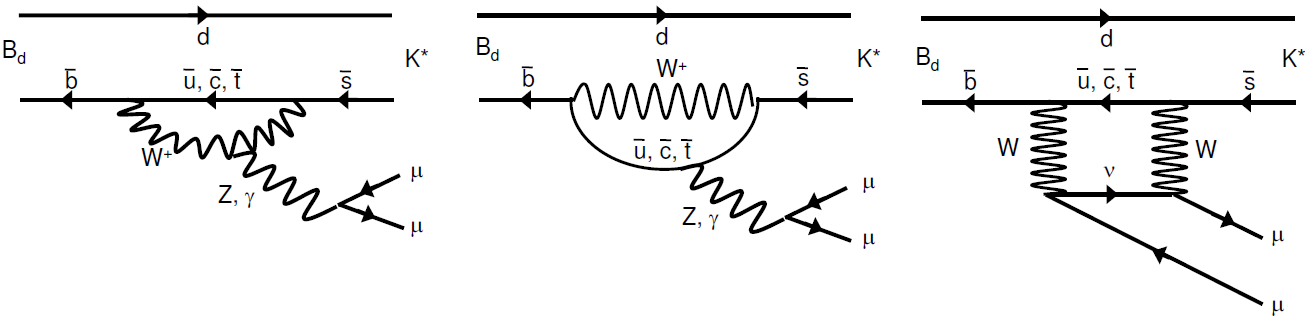
\includegraphics[width=0.66\columnwidth]{chapter2/figs/Feyn.png}
\caption[Feynman diagrams for a b to s transition]
{Three different Feynman diagrams showing the SM process that allow a \bsll transition,
 two penguin diagrams and a \W box diagram. ~\label{fig:bssm}}
\end{figure}
Processes which contain a \bquark\to\squark transition are popular FCNC decays for tests of contributions from new physics~\cite{Melikhov:1998cd}.
Measurements of FCNCs are model-independent tests of any new physics model that contribute to change the overall properties of the decay.

The formalism of \bquark-hadron decays can be expressed in terms of an effective theory, which separates different contributions to the decay 
by a particular mass scale. 
The effective theory of \B decays, Heavy Quark Effective Theory~\cite{Mannel:2004ce,Manohar:2000dt} ,
separates out particles with masses much greater than that of a \bquark quark, 
such as the electroweak gauge bosons, the Higgs, the \tquark quark and any new massive particles.
The operator product expansion separates these high and low energy contributions into a set of coefficients and operators~\cite{Wilson:1972ee},
\begin{align}
\bra{f}\mathcal{H}\ket{i} &=  \sum_k \C{k}(\mu) \bra{f}\Ope{k} (\mu)\ket{i}  \, ,
\end{align}
where the Wilson coefficients ($C$) and the operators ($O$) are normalised to a mass scale ($\mu$).

The operators encode the low energy contributions from the quarks in the decay and the Wilson coefficients encode
 the contributions from higher mass particles above the mass scale $\mu$.
For this reason the Wilson coefficients are said to encode the `short' distance physics whilst the 
operators encode the `long' distance physics.
The short distance physics covers everything above the mass scale of the effective Hamiltonian, 
such weak interactions and any contribution from physics beyond the SM.
The long distance physics covers everything below the mass scale of the Hamiltonian, 
\ie~the \Kstar physics and the interactions with the light spectator quark.
The benefit of this formalism is that the Wilson coefficients can include arbitrary contributions from new physical models and 
provide a model-independent formalism through which to measure these contributions.

The effective Hamiltonian for the \bsll transition~\cite{AltmannshoferBall} is
\begin{align}
H = \frac{4G_F}{\sqrt{2}} V_{tb}^{*} V_{ts} \sum_{i=1}^{10} C_i(\mu) O_i(\mu) \, .
\end{align}
The electroweak penguin operators are 
\begin{subequations}\begin{align}
\Ope{7}  &= \frac{e}{g^2}  m_b\left(\bar{\squark}\sigma_{\mu\nu}\frac{1}{2}(1\pm\gamma^5)\bquark\right) F^{\mu\nu}   \, , \\
\Ope{8}  &= \frac{1}{g} m_b\left(\bar{\squark}\sigma_{\mu\nu}T^a\frac{1}{2}(1\pm\gamma^5)\bquark\right) G^{a,\mu\nu}   \, , \\
\Ope{9}  &= \frac{e^2}{g^2} m_b\left(\bar{\squark}\gamma_\mu\frac{1}{2}(1\mp\gamma^5)\bquark\right) (\bar{\ell} \gamma^\mu \ell ) \, , \\
\Ope{10}  &= \frac{e^2}{g^2} m_b\left(\bar{\squark}\gamma_\mu\frac{1}{2}(1\mp\gamma^5)\bquark\right) (\bar{\ell} \gamma^\mu \gamma^5 \ell ) \, ,
\end{align}\end{subequations}
where $g$ is the strong coupling constant and $m_b$ is the \bquark mass dependent on the chosen renormalisation scheme.
The operator \Ope7  describes the electroweak penguin decay with a photon propagator, \Ope8 describes the diagram with a gluon propagator 
and the operators \Ope9 and \Ope10 describe the diagrams with electroweak bosons, either \Wpm or \Z.
The respective Wilson coefficients for these quark transitions are \C7 , \C8 , \C9 and \C{10} ~\cite{Bobeth:1999mk}.
The Wilson coefficients at the \bquark mass are evolved down from the weak mass scale, giving effective Wilson coefficients which also
include contributions from the four-quark and gluonic operators \C{1\to6},
\begin{align}
\Ceff7 &= \frac{4\pi}{\alpha_S} \C7 - \frac{1}{3} \C3 - \frac{4}{9} \C4 - \frac{20}{3} \C5 - \frac{80}{9} \C6 , \\
\Ceff8 &= \frac{4\pi}{\alpha_S} \C8 + \C3 - \frac{1}{6} \C4 + 20 \C5 - \frac{10}{3} \C6 , \\
\Ceff9 &= \frac{4\pi}{\alpha_S} \C9 + Y(\qsq) \\
\Ceff10 &= \frac{4\pi}{\alpha_S}\C{10} \\
\Ceff_{7,8,9,10} &= \frac{4\pi}{\alpha_S}\Cpeff{7,8,9,10} \, .
\end{align}
where Y(\qsq), along with more detail about the effective coefficients can be found in Ref~\cite{AltmannshoferBall}.
Contributions from physics beyond the SM can also be parameterised in terms of the Wilson coefficients.
Right handed currents for each operator can be introduced as primed counterparts to the SM Wilson coefficients (\Cp{7}, \Cp{8}, \Cp{9} and \Cp{10} ) and 
 contributions from new scalars and pseudoscalar particles can be incorporated in the form of additional Wilson coefficients \C{S} and \C{P} .

Constraints on the Wilson coefficients can be obtained from measurements of different FCNCs~\cite{Altmannshofer:2012az}.
Measurements of \btosgam transitions are proportional to the magnitude of \C{7} and measurements of 
\bsll transitions in the form of \Bsmm are proportional the value of \C10 and could incorporate contributions from \C{S} and \C{P} .
The \bsll electroweak penguin decay is mainly parameterised by \C{7}, \C9 and \C{10} , allowing 
 measurements of the \bsll decays to constrain a wide range of models of physics beyond the SM.

%Theoretical predictions for each of the Wilson coefficients come from several methods depending on the energy given to 
%the \ellell and \kpi pair.
%For the energy region where the \Kstarz meson carries a large proportion of the available energy,
% the `large recoil' region, a technique called QCD factorisation can be used~\cite{Beneke:2000wa}.
% \emph{ QCD factorisation does something I still don't understand }
%There are two other regions, the dimuon range close to the charmonium (\jpsi and \psitwos) resonances 
% and the limit of soft \Kstarz and high momentum dimuon where two different approaches must be taken, as described in 
% Refs~\cite{Khodjamirian:2010vf} and~\cite{Bobeth:2011nj} respectively.




\section{Experimental results}

The first measurement of a \bquark\to\squark FCNC was the \btosgam transition observed in the measurement of the branching fraction of \decay{\B}{\Kstar\g} at \cleo in 1993~\cite{PhysRevLett.71.674}.
\BdKstGam is a radiative electroweak penguin decay described by the photon operator \Ope7 and hence is sensitive to \C7 .
Subsequent precision measurements of \BdKstGam and 
the similar decay \BsPhiGam have been performed by the B factories, \babar~\cite{babar:exp-b2kstgamma:2009} 
and \belle~\cite{PhysRevLett.103.241801} along with \lhcb~\cite{LHCb-PAPER-2011-042,LHCb-PAPER-2012-019,LHCb-CONF-2012-004}.
These measurements of the differential branching fraction of \BdKstGam, \BsPhiGam and measurements of 
the \CP asymmetry \ACP(\BdKstGam)~\cite{PDG2012} agree well with the predictions from the SM~\cite{hfag:2012,Ali:th-b2vgamma-NNLO:2008}.

The FCNC decay \BdToKstll was proposed as a further test for contribution from physics beyond the SM in Ref~\cite{PhysRevD.61.114028}.
However, the differential branching fraction of the inclusive decay \BdToKstll and the exclusive decay \BdToKstmm 
have been measured~\cite{hfag:2012} to be
\begin{align}
\Gamma(\BdToKstll) &= 9.9^{+1.2}_{-1.1} \times 10^{-7} \\
\Gamma(\BdToKstmm) &= 1.06\pm0.10 \times 10^{-6}
\end{align}
and are compatible with SM prediction~\cite{Ligeti:2007sn,Huber:2007vv}.

Further measurements of \BdToKstll are based on  evaluating the
angular distribution of the daughter particles to understand the \Kstarz polarisation amplitudes.
How to determine the maximal amount of information from the decay
while keeping uncertainties from QCD minimal has recently attracted much 
interest~\cite{Kruger:2005ep,Egede:2008uy,AltmannshoferBall,Egede:2010zc,Bobeth:2010wg,Matias:2012xw}.

The results from the experimental analyses of 
\BdToKstll~\cite{Aubert:2008ju,PhysRevLett.103.171801,Aaltonen:2011cn,Aaij:2011aa} 
have focused on the forward-backward asymmetry of the
dimuon system (\AFB) and the fraction of longitudinal polarisation of
the \Kstarz (\FL) as a function of the dimuon invariant mass.
The latest measurements from \babar, \belle and \cdf for \FL and \AFB are shown in Fig.~\ref{fig:otherexp}.
\begin{figure}[tbp]
\centering
\subfigure[\FL]{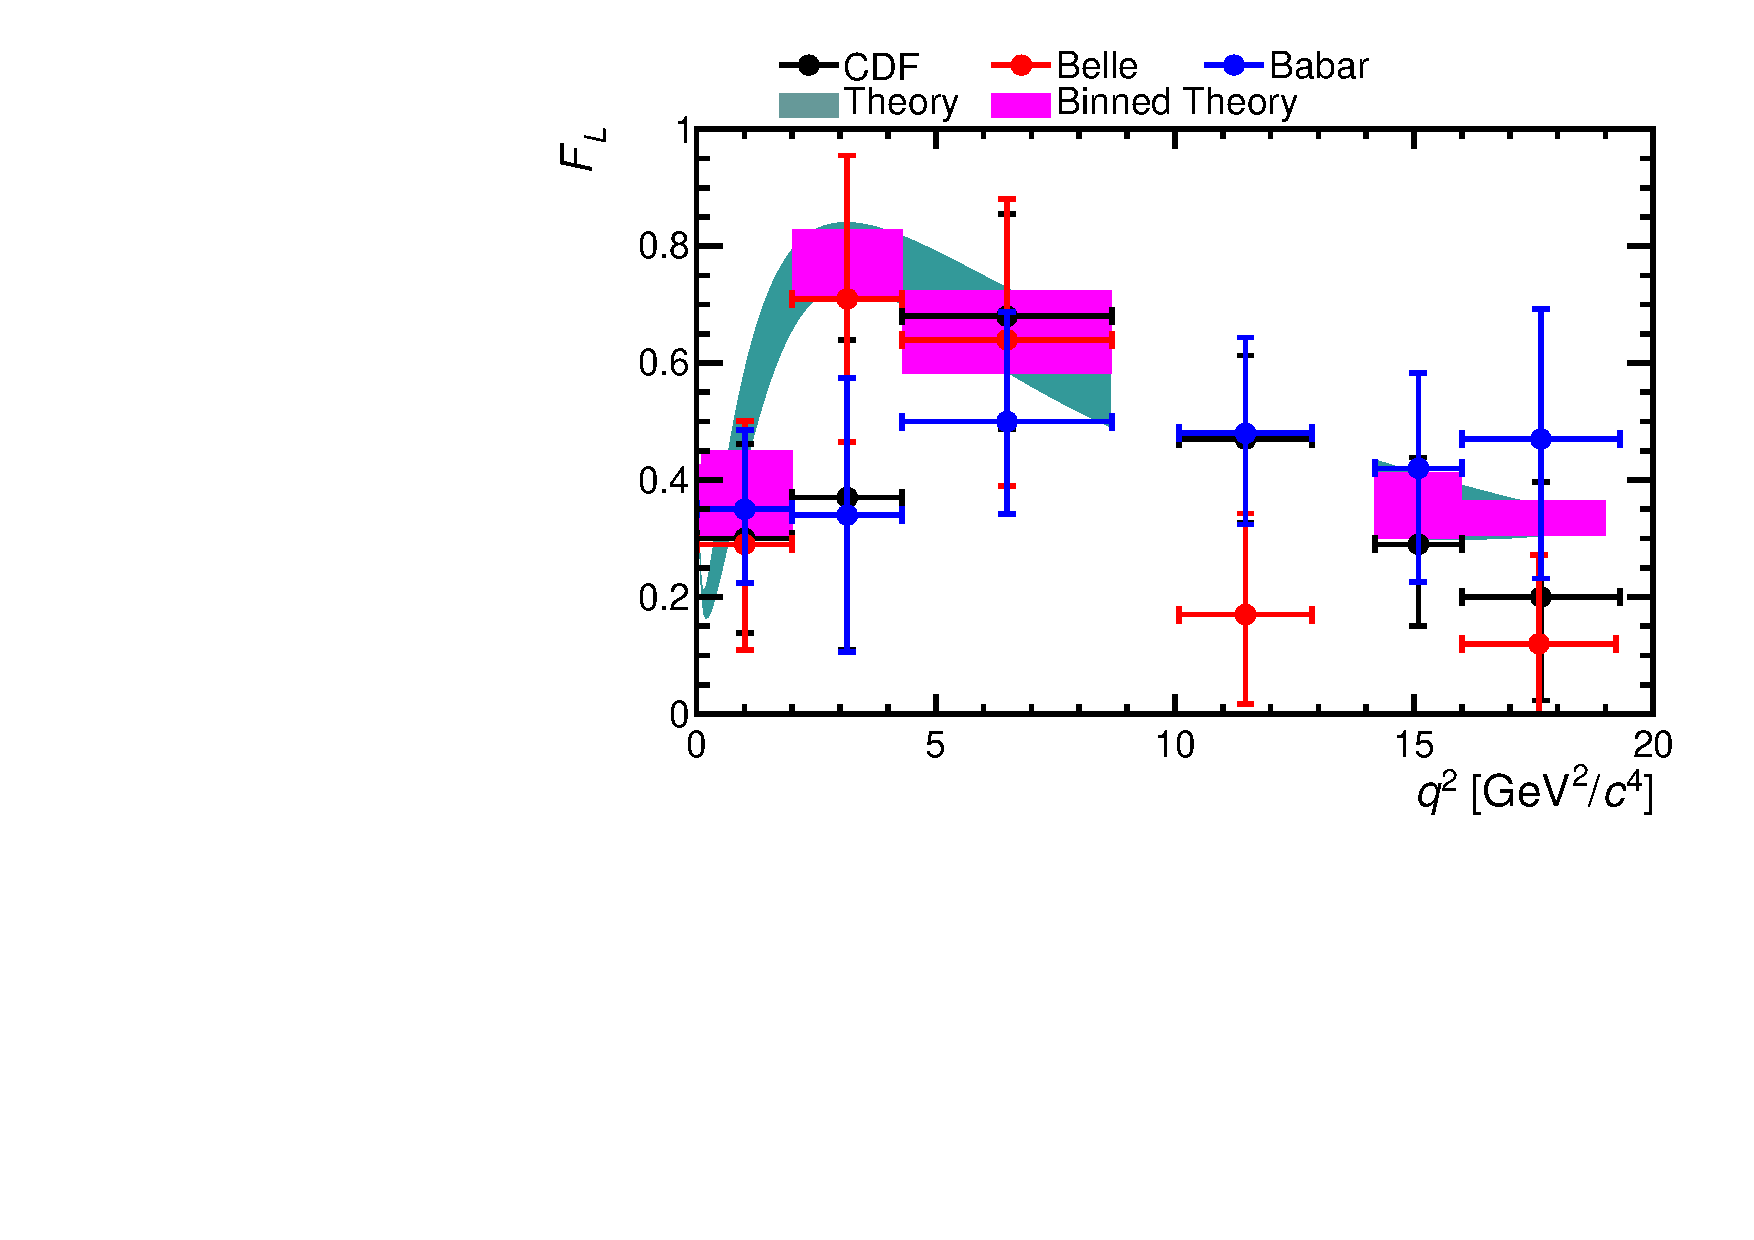
\includegraphics[width=0.48\columnwidth]{chapter2/figs/plot_FLExp.pdf}}
\subfigure[\AFB]{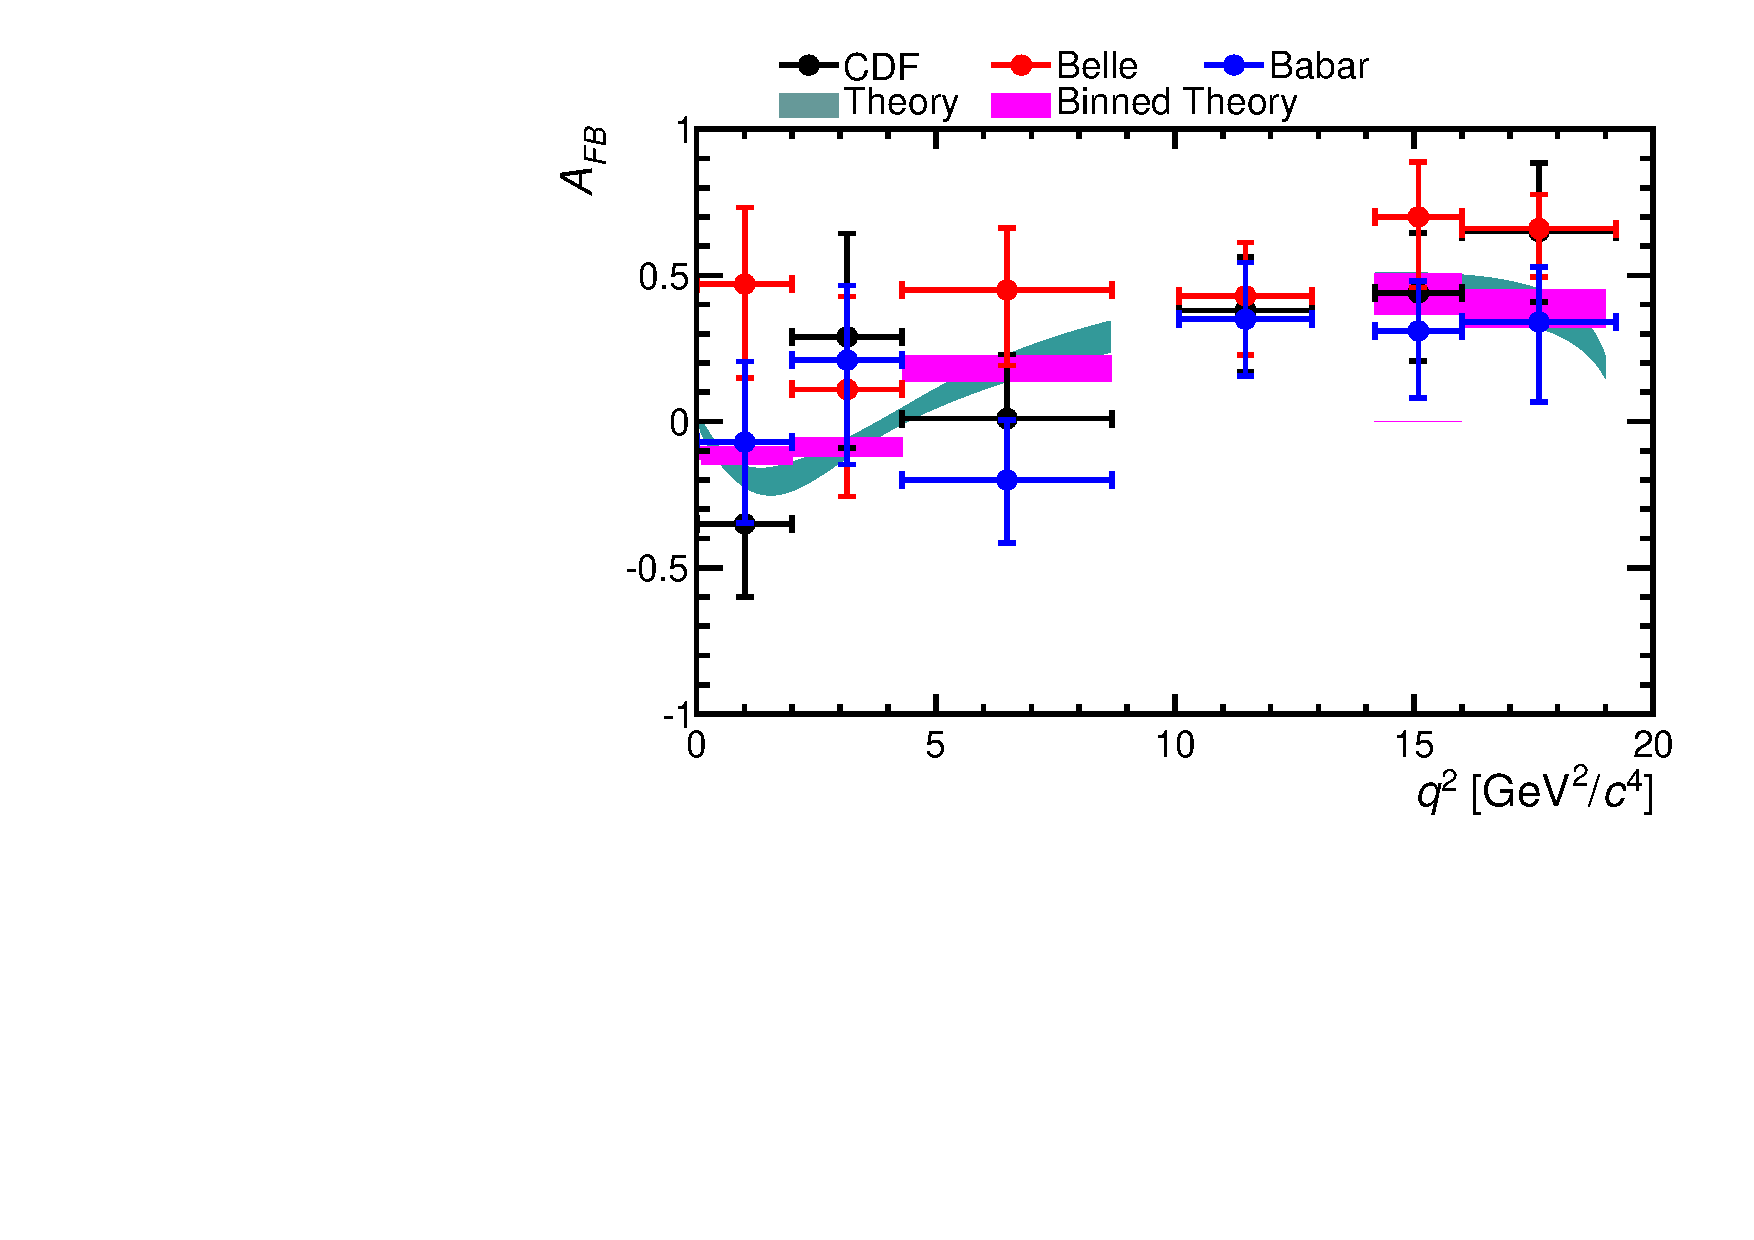
\includegraphics[width=0.48\columnwidth]{chapter2/figs/plot_AFBExp.pdf}}
\caption[\BdToKstmm measurements from \babar, \belle and \cdf]
{The fraction of longitudinal polarisation of the \Kstarz (\FL) and 
the  forward-backward asymmetry of the dimuon system (\AFB)  as measured by
\cdf~\cite{Aaltonen:2011cn,Aaltonen:2011ja}, \belle~\cite{PhysRevLett.103.171801} 
and \babar~\cite{Aubert:2007hz,Aubert:2008ju} 
along with the theoretical prediction from Ref.~\cite{Bobeth:2011gi}.~\label{fig:otherexp} }
\end{figure}
It is possible to see that there is some tension between these measurements of both \FL and \AFB at low dimuon invariant masses.
Contributions from physics beyond the SM have been predicted to change the \qsq spectrum of  \AFB~\cite{Egede:2010zc} which are not excluded by these measurements.
New measurements of \FL and \AFB are  needed to understand the exact shape of \AFB and clarify the discrepancy in the regions of low and high \qsq.
%In this thesis, the world-best measurements of the angular observables of \BdToKstmm using data from the \lhcb experiment presented along with 
%new measurements of the \kpi system.% do help understanding of the result of current and future angular analyses.

